%\thesistitle{
%    Sweet Little Nothings: Searching for a Pairs of Supersymmetric Tops,
%        a Pair of Higgs Bosons, and a Pair of New Small Wheels for the 
%        Upgrade of the ATLAS Forward Muon System
%}

\thesistitle{
Searches for Anomalous Resonances in the Large Hadron Collider for New Physics
}

%"Dissertation" for PhD, "Thesis" for master's
\documenttitle{Dissertation}

\degreename{Doctor of Philosophy}

% Use the wording given in the official list of degrees awarded by UCI:
% http://www.rgs.uci.edu/grad/academic/degrees_offered.htm
\degreefield{
Physics
}

% Your name as it appears on official UCI records.
\authorname{
Yvonne Ng
}

% Use the full name of each committee member.
\committeechair{Professor Daniel Whiteson}
\othercommitteemembers
{
  Professor Tim Tait\\
  Professor Andrew Lankford
}

\degreeyear{2021}

\copyrightdeclaration
{
  {\copyright} {\Degreeyear} \Authorname
}

% If you have previously published parts of your manuscript, you must list the
% copyright holders; see Section 3.2 of the UCI Thesis and Dissertation Manual.
% Otherwise, this section may be omitted.
% \prepublishedcopyrightdeclaration
% {
% 	Chapter 4 {\copyright} 2003 Springer-Verlag \\
% 	Portion of Chapter 5 {\copyright} 1999 John Wiley \& Sons, Inc. \\
% 	All other materials {\copyright} {\Degreeyear} \Authorname
% }

% The dedication page is optional
% (comment out to exclude).
\dedications
{
  (Optional dedication page)
  
  To ...
}

\acknowledgments
{
     First of all, I would like to thank my advisor Daniel Whiteson and Andy Lankford for the guidance, support, trust, and freedom they have given me over the years. I am especially grateful for Daniel's continuous encouragement towards my growth into an independent researcher. 

I would also like to thank my postdocs Dan Guest and Mike Fenton. Thank you for all the big and small advice on my work and personal encouragements over the years- sometime in the form of French Kabob runs or pandemic zoom coffees sessions. A special thank you is also dedicated to Kate Pachal, for your generous support through my first major analysis, for teaching me so much that I know now, and for the afternoon cake time at R1. I will strive to be like what you all were to me to my future students.

I am grateful for my colleagues at CERN, especially Verena Martinez, Bill Murray, Ben Nachman, Bogdan Malaescu, Caterina Doglioni, Christopher Haynes, Ljiljana Morvaj, Heather Russell, and Kyle Cranmer. The end product of this thesis would not have the same rigor without your technical comments and contributions.

A gratitude is also extended to my informal advisors in Irvine, Tim Tait, Muchun Chen, Simona Murgia, and Michael Ratz for the intellectual support and advice. I also want to thank Flip Tanedo for all the coffee and restaurant runs in my first two years of grad school. I was nourished in the mind, in my stomach, and also in my caffeine level. I also want to thank Chase and Seyda for all the thought-provoking chats.

If I am allowed the indulgence to take it back to where the journey begins, I want to thank my middle science teacher Miss Chau, thank you for always having so much trust in my abilities and for showing me how practical and relatable science is. I also want to thank my math teacher Miss Fung: for both the lessons in math and outside of math. Some words outside of math took me many years more years to understand after class was over. I am grateful to my undergraduate friends and
``Senpais" David and Jason, for showing me the fun of solving technical problems with science and engineering and for being great friends. I am also thankful for research time from MC Chu in his lab. I learned not just the rigor of scientific research but also responsibility as a scientist to society. I aspire to continue my efforts of scientific outreach as a postdoc like you have done for so many. 

%NAthan , Chase, seyda matt and jennifer, 
It only took 3 continents to finish my Ph.D. These would not have been possible without the support of my friends across all three continents. Special shout out to Andy, Clare, Diane, Haidee, Alexis, Ros, Yanyi, CY, Rhoda, Alice, Joakim, Lily, Arianna, Freida, Kit, Ho, Amber, Tamara, Kiwi, Shelly, Danny, friends in Kindle Hills. My life in the last few years both instead and outside of physics really wouldn't have been the same without you.

Finally to my family: mom and dad, I hope I made you proud. To my brother Rene, I am lucky to have your support and to have you as a partner in crime through all of life's adventures.

This thesis is for all of you.


%  I would like to thank...
%  
%  (You must acknowledge grants and other funding assistance. 
%  
%  You may also acknowledge the contributions of professors and
%  friends.
%  
%  You also need to acknowledge any publishers of your previous
%  work who have given you permission to incorporate that work
%  into your dissertation. See Section 3.2 of the UCI Thesis and
%  Dissertation Manual.)
}


% Some custom commands for your list of publications and software.
\newcommand{\mypubentry}[3]{
  \begin{tabular*}{1\textwidth}{@{\extracolsep{\fill}}p{4.5in}r}
    \textbf{#1} & \textbf{#2} \\ 
    \multicolumn{2}{@{\extracolsep{\fill}}p{.95\textwidth}}{#3}\vspace{6pt} \\
  \end{tabular*}
}
\newcommand{\mysoftentry}[3]{
  \begin{tabular*}{1\textwidth}{@{\extracolsep{\fill}}lr}
    \textbf{#1} & \url{#2} \\
    \multicolumn{2}{@{\extracolsep{\fill}}p{.95\textwidth}}
    {\emph{#3}}\vspace{-6pt} \\
  \end{tabular*}
}

% Include, at minimum, a listing of your degrees and educational
% achievements with dates and the school where the degrees were
% earned. This should include the degree currently being
% attained. Other than that it's mostly up to you what to include here
% and how to format it, below is just an example.
%
% CV is required for PhD theses, but not Master's
% comment out to exclude
\curriculumvitae
{
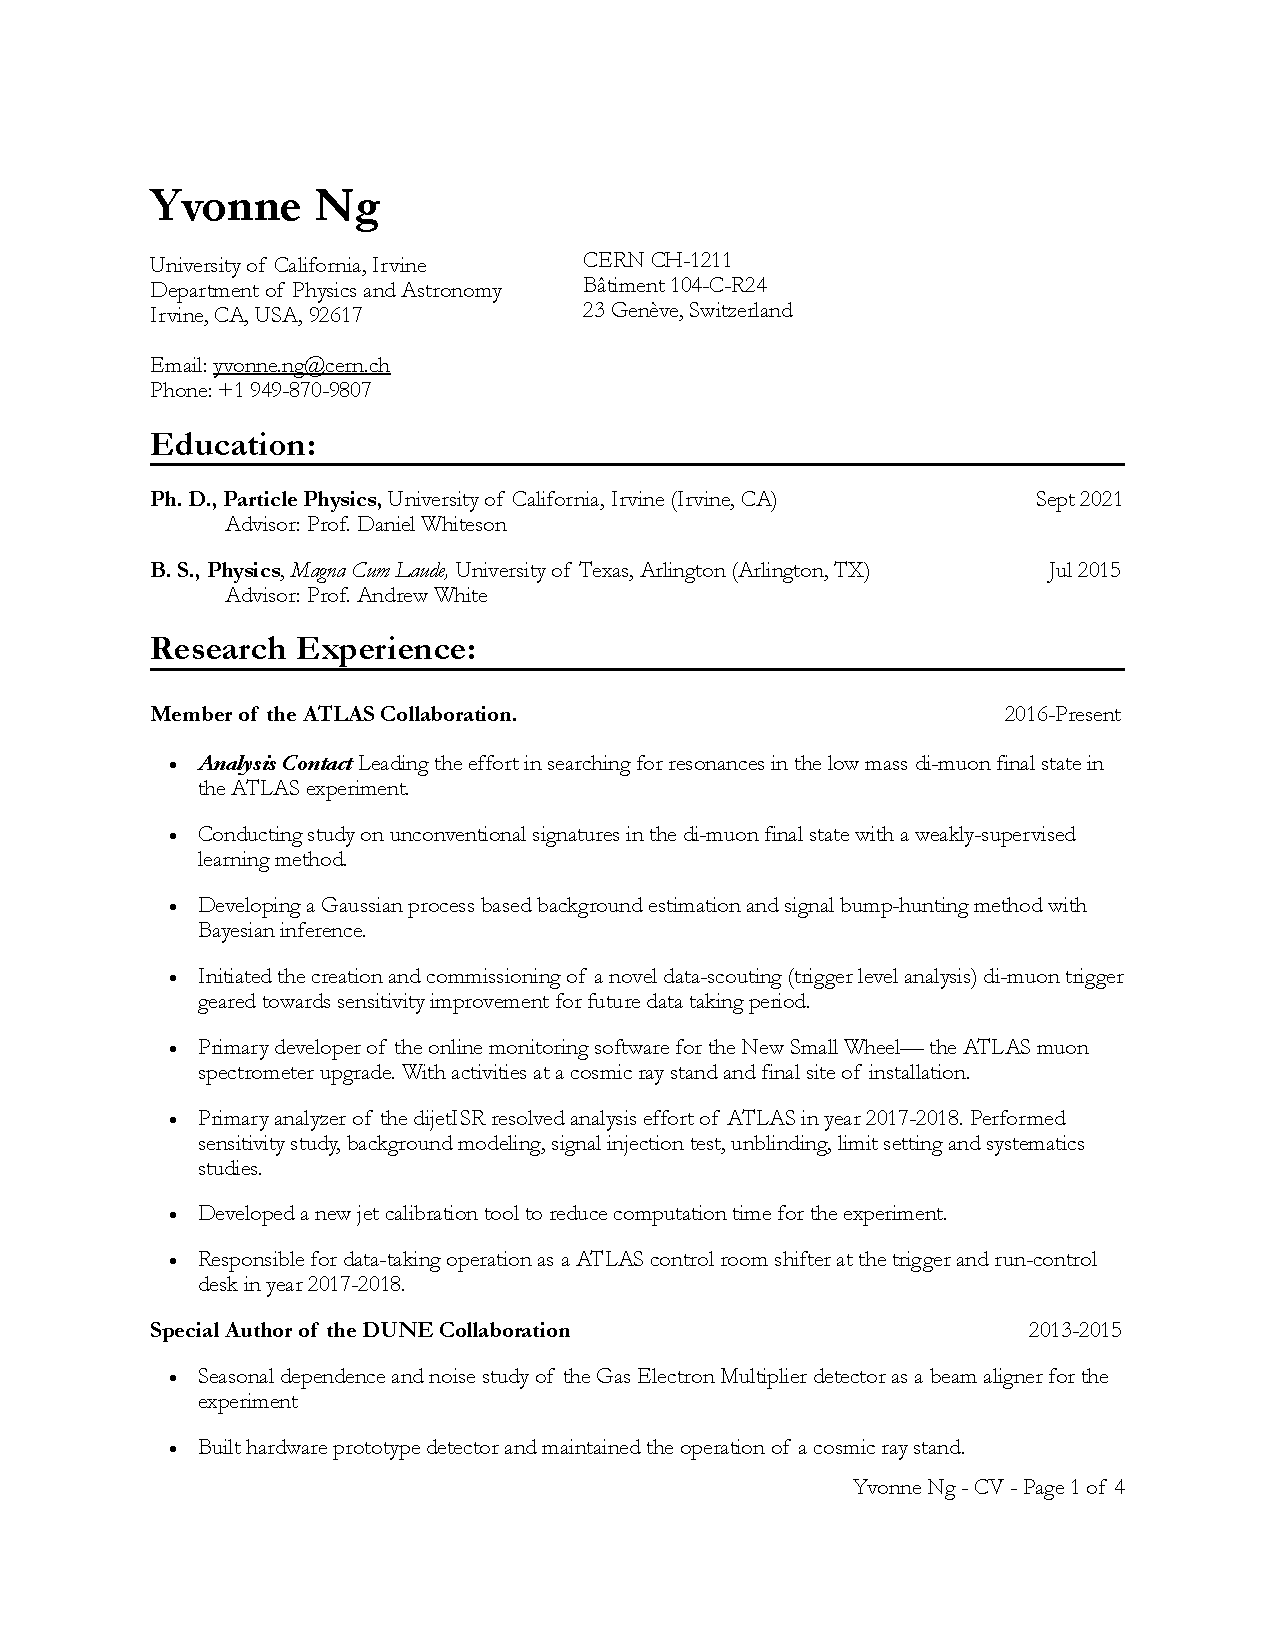
\includepdf[pages=-]{/Users/yvonne/WorkSpace/phd_thesis/phd_thesis/thesis/misc_metadata/cv/YWYvonneNg_CV_FermiLab.pdf}



%\textbf{EDUCATION}
%  
%  \begin{tabular*}{1\textwidth}{@{\extracolsep{\fill}}lr}
%    \textbf{Doctor of Philosophy in Computer Science} & \textbf{2012} \\
%    \vspace{6pt}
%    University name & \emph{City, State} \\
%    \textbf{Bachelor of Science in Computational Sciences} & \textbf{2007} \\
%    \vspace{6pt}
%    Another university name & \emph{City, State} \\
%  \end{tabular*}
%
%\vspace{12pt}
%\textbf{RESEARCH EXPERIENCE}
%
%  \begin{tabular*}{1\textwidth}{@{\extracolsep{\fill}}lr}
%    \textbf{Graduate Research Assistant} & \textbf{2007--2012} \\
%    \vspace{6pt}
%    University of California, Irvine & \emph{Irvine, California} \\
%  \end{tabular*}
%
%\vspace{12pt}
%\textbf{TEACHING EXPERIENCE}
%
%  \begin{tabular*}{1\textwidth}{@{\extracolsep{\fill}}lr}
%    \textbf{Teaching Assistant} & \textbf{2009--2010} \\
%    \vspace{6pt}
%    University name & \emph{City, State} \\
%  \end{tabular*}
%
%\pagebreak
%
%\textbf{REFEREED JOURNAL PUBLICATIONS}
%
%  \mypubentry{Ground-breaking article}{2012}{Journal name}
%
%\vspace{12pt}
%\textbf{REFEREED CONFERENCE PUBLICATIONS}
%
%  \mypubentry{Awesome paper}{Jun 2011}{Conference name}
%  \mypubentry{Another awesome paper}{Aug 2012}{Conference name}
%
%\vspace{12pt}
%\textbf{SOFTWARE}
%
%  \mysoftentry{Magical tool}{http://your.url.here/}
%  {C++ algorithm that solves TSP in polynomial time.}
%
}

% The abstract was previously limited to a maximum of 350 words, 
% but the UCI manual at https://etd.lib.uci.edu/electronic/td2e#2.2.1.
% currently does not indicate that there is any word limit for the abstract
\thesisabstract
{
  Many empirical evidence points to the existence of beyond-the-standard-model physics. In the LHC, different theoretical and experiemntal tehcniques are used to look for new particles as for new physics. One method with theoretical elegance and clean experimental reconstruction, is the resonance finding method. The method has enjoyed much sucesses in the past, W, Z and the Higgs boson are some of the few particles discovered this way. However, the early beyond-the-standard-model resonance search program of the LHC has returned empty handed. 
In this thesis, I ask the question of whether the standard approach could be modified to look for "weird resonances", particles that exist in the LHC dataset but goes beyond the standard program. Their discovery can provide important clue to beyond-the-standard-model physics. 

Three physics analyses beyond the usual search program are covered in this thesis. The first two on the dijetISR final state and the last one on dimuon final state. In the dijetISR searches, an ISR object is used to boost the final state. By triggering on the ISR object rather than the resonance formming final state, lower mass resonances can be covered. These two analysis set the lowest ATLAS low mass limit below the standard dijet search. In the dimuon search, as previous searches has neglected the low mass region below the Z peak, the search seeks to cover the region from 12-70 GeV. A novel statistical method driven by Gaussian Process is used. The method allow for a simple background estimation for a similar class of future analyses where Monte Carlo is limited.

All of these analyses provide competitive exclusion in the dark matter benchmark model of the LHC in places not previously covered.

As a future discussion, a new stream from trigger level analysis could be implemented to the dimuon search to improve the low mass sensitivity. Data driven approach like CWOLA can also be used to look for resonances free of an assumed signal model.

The thesis also covers involvement jet in-situ calibration as well as the new small wheel online monitoring software development.

"Weird resonances" are the "out-of-ordinary" ones: They are not a part of the current knowledge model; they break existing laws; they defies our knowledge about the world and human-beings; they are already somewhere out there, but only from its discovery it can be realized that we are more than what we think we are. The search for weird resonanances is a search for authenticity.

  %The abstract of your contribution goes here.
}


%%% Local Variables: ***
%%% mode: latex ***
%%% TeX-master: "thesis.tex" ***
%%% End: ***
